\documentclass{beamer}

% xcolor and define colors -------------------------
\usepackage{xcolor}

% https://www.viget.com/articles/color-contrast/
\definecolor{purple}{HTML}{5601A4}
\definecolor{navy}{HTML}{0D3D56}
\definecolor{ruby}{HTML}{9a2515}
\definecolor{alice}{HTML}{107895}
\definecolor{daisy}{HTML}{EBC944}
\definecolor{coral}{HTML}{F26D21}
\definecolor{kelly}{HTML}{829356}
\definecolor{cranberry}{HTML}{E64173}
\definecolor{jet}{HTML}{131516}
\definecolor{asher}{HTML}{555F61}
\definecolor{slate}{HTML}{314F4F}

% Mixtape Sessions
\definecolor{picton-blue}{HTML}{00b7ff}
\definecolor{violet-red}{HTML}{ff3881}
\definecolor{sun}{HTML}{ffaf18}
\definecolor{electric-violet}{HTML}{871EFF}

\newcommand\pictonBlue[1]{{\color{picton-blue}#1}}
\newcommand\sun[1]{{\color{sun}#1}}
\newcommand\electricViolet[1]{{\color{electric-violet}#1}}
\newcommand\violetRed[1]{{\color{violet-red}#1}}

\newcommand\bgPictonBlue[1]{{\colorbox{picton-blue!20!white}{#1}}}
\newcommand\bgSun[1]{{\colorbox{sun!20!white}{#1}}}
\newcommand\bgElectricViolet[1]{{\colorbox{electric-violet!20!white}{#1}}}
\newcommand\bgVioletRed[1]{{\colorbox{violet-red!20!white}{#1}}}

\def\code#1{\texttt{#1}}

% Main theme colors
\definecolor{accent}{HTML}{00b7ff}
\definecolor{accent2}{HTML}{871EFF}
\definecolor{gray100}{HTML}{f3f4f6}
\definecolor{gray800}{HTML}{1F292D}


% Beamer Options -------------------------------------

% Background
\setbeamercolor{background canvas}{bg = white}

% Change text margins
\setbeamersize{text margin left = 15pt, text margin right = 15pt} 

% \alert
\setbeamercolor{alerted text}{fg = accent2}

% Frame title
\setbeamercolor{frametitle}{bg = white, fg = jet}
\setbeamercolor{framesubtitle}{bg = white, fg = accent}
\setbeamerfont{framesubtitle}{size = \small, shape = \itshape}

% Block
\setbeamercolor{block title}{fg = white, bg = accent2}
\setbeamercolor{block body}{fg = gray800, bg = gray100}

% Title page
\setbeamercolor{title}{fg = gray800}
\setbeamercolor{subtitle}{fg = accent}

%% Custom \maketitle and \titlepage
\setbeamertemplate{title page}
{
    %\begin{centering}
        \vspace{20mm}
        {\Large \usebeamerfont{title}\usebeamercolor[fg]{title}\inserttitle}\\
        {\large \itshape \usebeamerfont{subtitle}\usebeamercolor[fg]{subtitle}\insertsubtitle}\\ \vspace{10mm}
        {\insertauthor}\\
        {\color{asher}\small{\insertdate}}\\
    %\end{centering}
}

% Table of Contents
\setbeamercolor{section in toc}{fg = accent!70!jet}
\setbeamercolor{subsection in toc}{fg = jet}

% Button 
\setbeamercolor{button}{bg = accent}

% Remove navigation symbols
\setbeamertemplate{navigation symbols}{}

% Table and Figure captions
\setbeamercolor{caption}{fg=jet!70!white}
\setbeamercolor{caption name}{fg=jet}
\setbeamerfont{caption name}{shape = \itshape}

% Bullet points

%% Fix spacing between items
\let\olditemize=\itemize 
\let\endolditemize=\enditemize 
\renewenvironment{itemize}{\vspace{0.25em}\olditemize \itemsep0.25em}{\endolditemize}

%% Fix left-margins
\settowidth{\leftmargini}{\usebeamertemplate{itemize item}}
\addtolength{\leftmargini}{\labelsep}

%% enumerate item color
\setbeamercolor{enumerate item}{fg = accent}
\setbeamerfont{enumerate item}{size = \small}
\setbeamertemplate{enumerate item}{\insertenumlabel.}

%% itemize
\setbeamercolor{itemize item}{fg = accent!70!white}
\setbeamerfont{itemize item}{size = \small}
\setbeamertemplate{itemize item}[circle]

%% right arrow for subitems
\setbeamercolor{itemize subitem}{fg = accent!60!white}
\setbeamerfont{itemize subitem}{size = \small}
\setbeamertemplate{itemize subitem}{$\rightarrow$}

\setbeamertemplate{itemize subsubitem}[square]
\setbeamercolor{itemize subsubitem}{fg = jet}
\setbeamerfont{itemize subsubitem}{size = \small}








% Links ----------------------------------------------

\usepackage{hyperref}
\hypersetup{
  colorlinks = true,
  linkcolor = accent2,
  filecolor = accent2,
  urlcolor = accent2,
  citecolor = accent2,
}


% Line spacing --------------------------------------
\usepackage{setspace}
\setstretch{1.35}


% \begin{columns} -----------------------------------
\usepackage{multicol}


% Fonts ---------------------------------------------
% Beamer Option to use custom fonts
\usefonttheme{professionalfonts}

% \usepackage[utopia, smallerops, varg]{newtxmath}
% \usepackage{utopia}
\usepackage[sfdefault,light]{roboto}

% Small adjustments to text kerning
\usepackage{microtype}



% Remove annoying over-full box warnings -----------
\vfuzz2pt 
\hfuzz2pt


% Table of Contents with Sections
\setbeamerfont{myTOC}{series=\bfseries, size=\Large}
\AtBeginSection[]{
        \frame{
            \frametitle{Roadmap}
            \tableofcontents[current]   
        }
    }


% Tables -------------------------------------------
% Tables too big
% \begin{adjustbox}{width = 1.2\textwidth, center}
\usepackage{adjustbox}
\usepackage{array}
\usepackage{threeparttable, booktabs, adjustbox}
    
% Fix \input with tables
% \input fails when \\ is at end of external .tex file
\makeatletter
\let\input\@@input
\makeatother

% Tables too narrow
% \begin{tabularx}{\linewidth}{cols}
% col-types: X - center, L - left, R -right
% Relative scale: >{\hsize=.8\hsize}X/L/R
\usepackage{tabularx}
\newcolumntype{L}{>{\raggedright\arraybackslash}X}
\newcolumntype{R}{>{\raggedleft\arraybackslash}X}
\newcolumntype{C}{>{\centering\arraybackslash}X}

% Figures

% \imageframe{img_name} -----------------------------
% from https://github.com/mattjetwell/cousteau
\newcommand{\imageframe}[1]{%
    \begin{frame}[plain]
        \begin{tikzpicture}[remember picture, overlay]
            \node[at = (current page.center), xshift = 0cm] (cover) {%
                \includegraphics[keepaspectratio, width=\paperwidth, height=\paperheight]{#1}
            };
        \end{tikzpicture}
    \end{frame}%
}

% subfigures
\usepackage{subfigure}


% Highlight slide -----------------------------------
% \begin{transitionframe} Text \end{transitionframe}
% from paulgp's beamer tips
\newenvironment{transitionframe}{
    \setbeamercolor{background canvas}{bg=accent!40!black}
    \begin{frame}\color{accent!10!white}\LARGE\centering
}{
    \end{frame}
}


% Table Highlighting --------------------------------
% Create top-left and bottom-right markets in tabular cells with a unique matching id and these commands will outline those cells
\usepackage[beamer,customcolors]{hf-tikz}
\usetikzlibrary{calc}
\usetikzlibrary{fit,shapes.misc}

% To set the hypothesis highlighting boxes red.
\newcommand\marktopleft[1]{%
    \tikz[overlay,remember picture] 
        \node (marker-#1-a) at (0,1.5ex) {};%
}
\newcommand\markbottomright[1]{%
    \tikz[overlay,remember picture] 
        \node (marker-#1-b) at (0,0) {};%
    \tikz[accent!80!jet, ultra thick, overlay, remember picture, inner sep=4pt]
        \node[draw, rectangle, fit=(marker-#1-a.center) (marker-#1-b.center)] {};%
}


% DAGS ----------------------------------------------
\usepackage{tikz}
\usetikzlibrary{shapes,decorations,arrows,calc,arrows.meta,fit,positioning}
% Tikz settings optimized for causal graphs.
\tikzset{
    -Latex,auto,node distance =1 cm and 1 cm,semithick,
    state/.style ={ellipse, draw, minimum width = 0.7 cm},
    point/.style = {circle, draw, inner sep=0.04cm,fill,node contents={}},
    bidirected/.style={Latex-Latex,dashed},
    el/.style = {inner sep=2pt, align=left, sloped}
}


% Beamer tricks -------------------------------------
% Make \pause work in align environments
\makeatletter
\renewrobustcmd{\beamer@@pause}[1][]{%
  \unless\ifmeasuring@%
  \ifblank{#1}%
    {\stepcounter{beamerpauses}}%
    {\setcounter{beamerpauses}{#1}}%
  \onslide<\value{beamerpauses}->\relax%
  \fi%
}
\makeatother




\begin{document}

\imageframe{./lecture_includes/cover_hetero.png}

\section{The LATE Theorem}

\subsection{Potential Outcome Setup}
\begin{frame}{From Constant to Heterogeneous Effects}
So far we have implicitly been considering models w/ constant effects
\begin{itemize}
\item $Y_i=\alpha+\beta D_i+\varepsilon_i$ implies $\partial Y/\partial D = \beta$ for all observations $i$\smallskip
\item What if this model is \emph{misspecified}? I.e. what if $Y_i=\alpha+\beta_i D_i+\varepsilon_i$ ?
\end{itemize}\medskip\pause{}
Intuitively, different ``research designs'' (e.g. instruments) may capture different effects of the same treatment --- even when all are valid\smallskip
\begin{itemize}
\item Recall charter lottery vs. takeover IVs: very different setups!
\end{itemize}\medskip\pause{}
Formalized in the (Nobel-winning!) Imbens and Angrist '94 LATE thm.\smallskip
\begin{itemize}
\item Using a general potential outcomes framework...
\end{itemize}
\end{frame}

\begin{frame}{Potential Outcome Setup}
Let $Y_i(0)$ and $Y_i(1)$ denote individual $i$'s potential outcomes given a binary treatment $D_i\in\{0,1\}$\smallskip
\begin{itemize}
\item Observed outcomes: $Y_i=(1-D_i)Y_i(0)+D_iY_i(1)\pause{}=\alpha_i+\beta_i D_i$\smallskip\pause{}
\item Only observe one of these POs for each $i$; other is a \emph{counterfactual}\smallskip
\item Interested in the treatment effects $\beta_i=Y_i(1)-Y_i(0)$
\end{itemize}\medskip\pause{}
Imbens-Angrist' insight: we can also do this for an IV first stage:\smallskip
\begin{itemize}
\item Let $D_i(0)$ and $D_i(1)$ denote individual $i$'s potential \emph{treatment} given a binary \emph{instrument} $Z_i\in\{0,1\}$:\pause{} $D_i=(1-Z_i)D_i(0)+Z_i D_i(1)$\smallskip
\end{itemize}\medskip\pause{}
Under what assumptions can we causally interpret \code{ivreg2 Y (D=Z)}?
\end{frame}

\subsection{Theorem and Extensions}
\begin{frame}{Imbens and Angrist (1994) Assumptions}
\begin{enumerate}
\item \emph{As-good-as-random assignment}: $Z_i\perp (Y_i(0),Y_i(1),D_i(0),D_i(1))$\smallskip
\begin{itemize}
\item Consider the Angrist draft lottery, or Angrist-Krueger's QoB IV
\end{itemize}\medskip\pause{}
\item \emph{Exclusion}: $Z_i$ only affects $Y_i$ through its effect on $D_i$\smallskip
\begin{itemize}
\item Implicit in our potential outcomes notation: $Y_i(d)$ not indexed by $Z_i$
\end{itemize}\medskip\pause{}
\item \emph{Relevance}: $Z_i$ is correlated with $D_i$\smallskip
\begin{itemize}
\item Equivalently, given Assumption 1, $E[D_{i}(1)-D_i(0)]\neq 0$
\end{itemize}\medskip\pause{}
\item \emph{Monotonicity}: $D_{i}(1)\ge D_{i}(0)$ for all $i$ (i.e., almost-surely)\smallskip
\begin{itemize}
\item The instrument can only shift the treatment in one direction
\end{itemize}
\end{enumerate}
\end{frame}

\begin{frame}{Local Average Treatment Effect (LATE) Identification}
Imbens and Angrist showed that under these assumptions:
\begin{align*}
\beta^{IV}=E[Y_i(1)-Y_i(0)\mid D_i(1)>D_i(0)]
\end{align*}
\vspace{-0.6cm}

The IV estimand $\beta^{IV}$ identifies a LATE: the average treatment effect $Y_i(1)-Y_i(0)$ among \emph{compliers}: those with $1=D_i(1)>D_i(0)=0$\smallskip\pause{}
\begin{itemize}
\item Intuitively, IV can't tell us anything about the treatment effects of \emph{never-takers} $D_i(1)=D_i(0)=0$ / \emph{always-takers} $D_i(1)=D_i(0)=1$]\smallskip\pause{}
\item Monotonicity rules out the presence of \emph{defiers}, with $D_i(1)<D_i(0)$\pause{}
\end{itemize}\medskip
\begin{center}$\implies$Different (valid) IVs can identify different LATEs! \end{center}
\end{frame}

\begin{frame}{What Does This Mean \emph{Practically}?} 
Two conceptually distinct considerations: \emph{internal} vs. \emph{external} validity\smallskip
\begin{itemize}
\item Context of an IV, and who the compliers likely are, may matter\smallskip
\item Usual ``overidentification'' test logic fails: two valid IVs may have different estimands! (see Kitagawa (2015) for alternative tests)
\end{itemize}\medskip\pause{}
In addition to as-good-as-random assignment / exclusion, we may need to worry about monotonicity when we do IV\smallskip
\begin{itemize}
\item Sensible in earlier lottery / natural experiment / panel examples \smallskip
\item Maybe questionable in judge IVs (coming soon!)
\end{itemize}
\end{frame}


\begin{frame}{Extensions}
\vspace{-0.2cm}
Angrist and Imbens worked out the original LATE theroem for binary $D_i$, discrete $Z_i$, and no included controls\pause{}... but it extends\smallskip\pause{}
\begin{itemize}
\item Angrist/Imbens '95: multivalued (ordered) $D_i$, saturated covariates\smallskip
\item Angrist/Graddy/Imbens '00: continuous $D_i$ (supply/demand setup)\smallskip
\item Heckman/Vytlicil '05: continuous $Z_i$ (more on this soon)\smallskip
\item Multiple unordered treatments is harder (e.g. Behaghel et al. 2013)
\end{itemize}\medskip\pause{}
Recent discussions highlight importance of including flexible controls\smallskip
\begin{itemize}
\item E.g. Sloczy\'{n}ski '20, Borusyak and Hull '21, Mogstad et al. '22\smallskip
\item If monotonicity only holds conditional on $X_i$, may need $Z_i$-by-$X_i$ interactions (which may lead to many-weak problems...)
\end{itemize}
\end{frame}

\section{Characterizing Compliers}

\begin{frame}{Who Are the Compliers?}
Characterizing the $i$ that make up the IV estimand (w/$D_i(1)>D_i(0)$) is key for understanding internal vs. external validity \smallskip
\begin{itemize}
\item Unfortunately we can't identify compliers directly: we only observe $D_i(1)$ (when $Z_i=1$) or $D_i(0)$ (when $Z_i=0$), not both together!
\end{itemize}\bigskip\pause{}
It turns out we can still characterize compliers by their outcomes ($Y_i(0)$ and $Y_i(1)$) and other observables $X_i$\smallskip
\begin{itemize}
\item Comparing $E[X_i\mid D_i(1)>D_i(0)]$ to $E[X_i]$ can maybe shed light on how $E[Y_i(1)-Y_i(0)\mid D_i(1)>D_i(0)]$ compares to $E[Y_i(1)-Y_i(0)]$
\end{itemize}
\end{frame}

\subsection{Outcomes}
\begin{frame}{Outcomes}
Computing $E[Y_i(1)\mid D_i(1)>D_i(0)]$ is surprisingly easy in the IA setup\smallskip
\begin{itemize}
\item Define $W_i=Y_iD_i$, and note that this new outcome has potentials with respect to $D_i$ of $W_i(1)=Y_i(1)$ and $W_i(0)=0$\smallskip\pause{}
\item Thus IV with $W_i$ as the outcome identifies $E[W_i(1)-W_i(0)\mid D_i(1)>D_i(0)]=E[Y_i(1)\mid D_i(1)>D_i(0)]$
\end{itemize}\medskip\pause{}
Similar logic shows that IV with $Y_i(1-D_i)$ as the outcome and $1-D_i$ as the treatment identifies $E[Y_i(0)\mid D_i(1)>D_i(0)]$\smallskip
\begin{itemize}
\item So easy to do! And extends to covariates / multiple IVs...
\end{itemize}
\end{frame}

\begin{frame}{Characterizing Charter Lottery Complier $Y_i(0)$'s}
\begin{center}
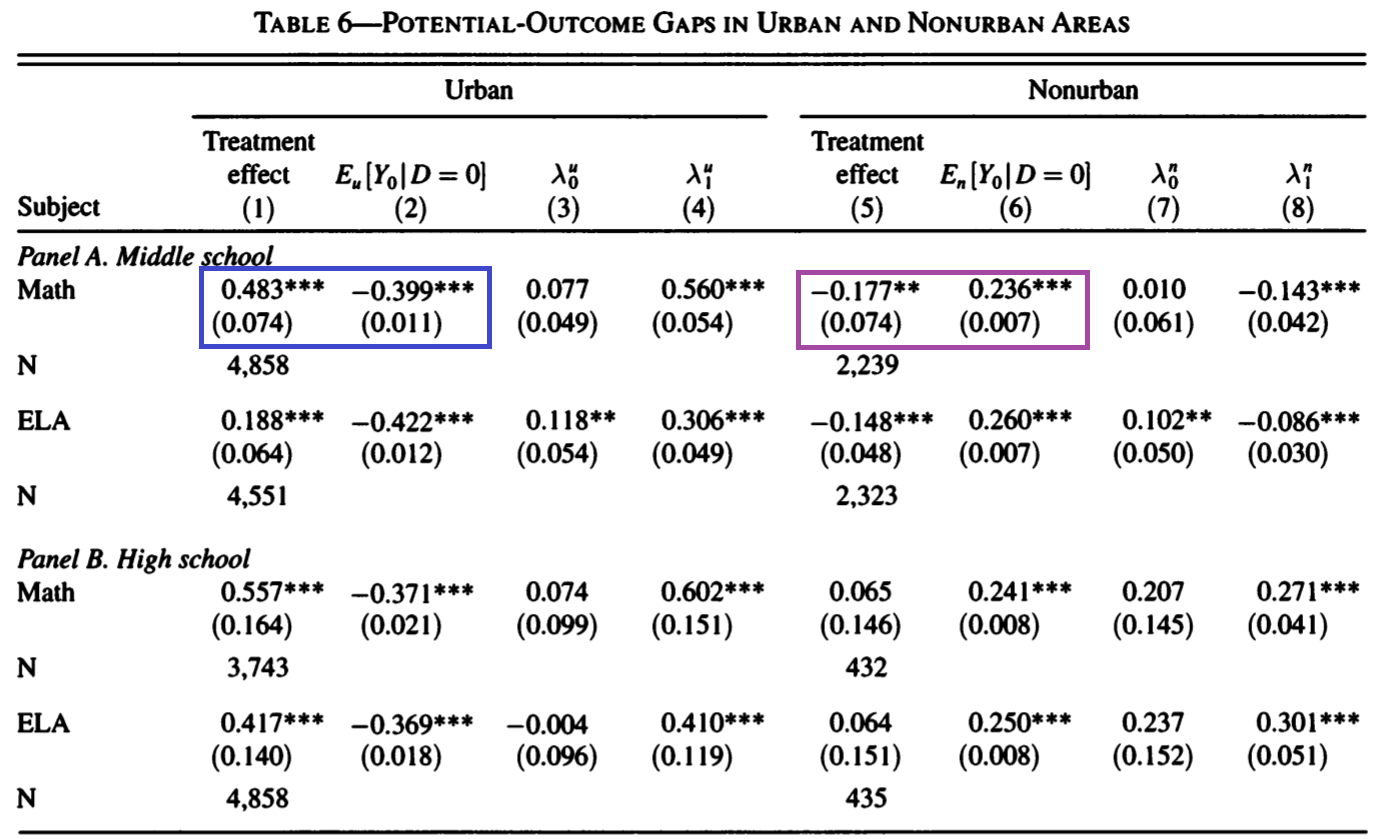
\includegraphics[scale=0.32]{./lecture_includes/cfx.png}
\end{center}
Source: Angrist, Pathak, and Walters (2013)
\end{frame}

\subsection{Covariates}
\vspace{-0.5cm}
\begin{frame}{Covariates}
For covariates $X_i$ (not affected by $D_i$) we can follow a similar trick:\smallskip
\begin{itemize}
\item Either IV'ing $X_iD_i$ on $D_i$ or IV'ing $X_i(1-D_i)$ on $1-D_i$ identifies complier characteristics $E[X_i\mid D_i(1)>D_i(0)]$\smallskip
\item Shouldn't be very different (implicit balance test); can be averaged
\end{itemize}\bigskip\pause{}
Abadie (2003) gives a slicker (but a bit more involved) approach to estimating any function of $(Y_i(0),Y_i(1),X_i)$ for compliers\smallskip
\begin{itemize}
\item Involves weighting by $\kappa=1-\frac{D_i(1-Z_i)}{1-E[Z_i\mid W_i]}-\frac{(1-D_i)Z_i}{E[Z_i\mid W_i]}$ where $W_i$ are any necessary ``design controls'' (e.g. lottery risk sets)\smallskip
\item You can do some really cool stuff with this!
\end{itemize}
\end{frame}

\begin{frame}{Black/White Potential Outcomes, Pre-Charter}
\vspace{-0.5cm}
\begin{center}
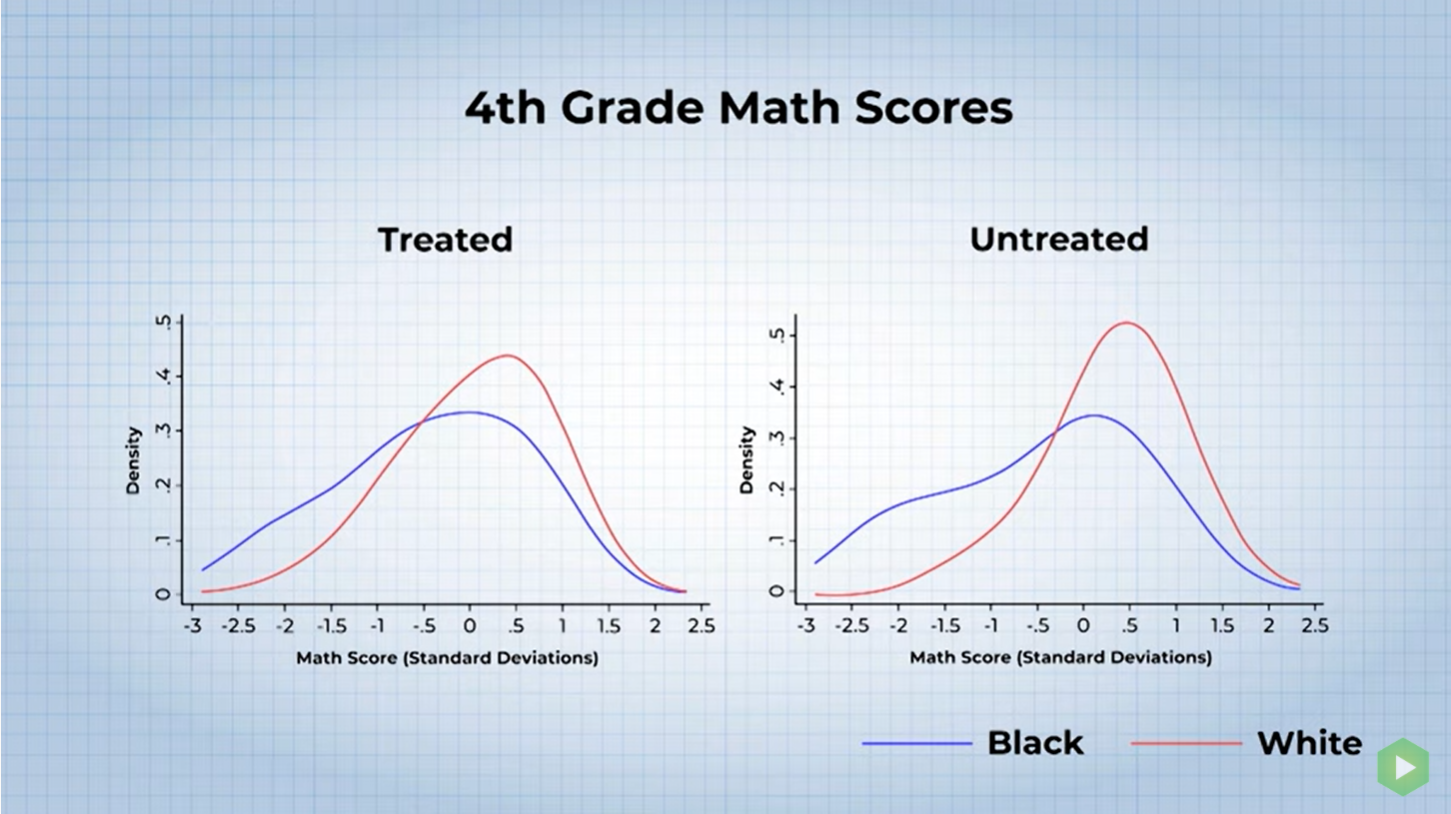
\includegraphics[scale=0.3]{./lecture_includes/angrist_distribution_4.png}
\end{center}
Source: Josh Angrist Nobel Lecture (2021) 
\end{frame}

\begin{frame}{Black/White Potential Outcomes, Post-Charter}
\vspace{-0.5cm}
\begin{center}
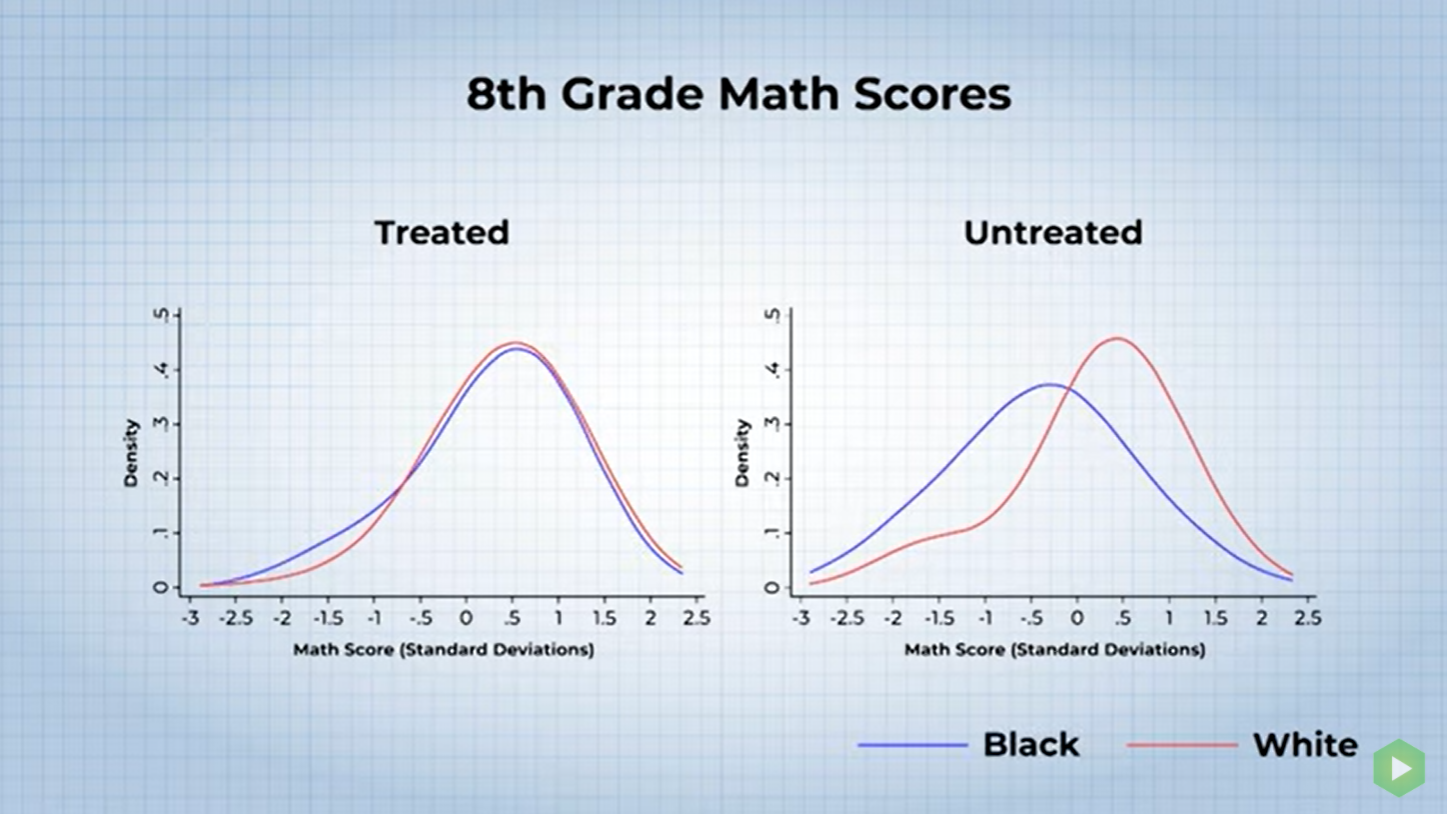
\includegraphics[scale=0.3]{./lecture_includes/angrist_distribution_8.png}
\end{center}
Source: Josh Angrist Nobel Lecture (2021) 
\end{frame}

\section{Marginal Treatment Effects}

\subsection{Continuous Instruments}
\begin{frame}{Heckman and Vytlicil (2005, 2007, 2010, 2013...)}
If we have a $Z_i$ that varies continuously, we might learn more about how treatment effects vary with compliance \smallskip
\begin{itemize}
\item Different types of $i$ may ``respond'' at different margins of $Z_i$
\end{itemize}\medskip\pause{}
Heckman-Vytlicil write $D_i=\mathbf{1}[p(Z_i)\ge U_i]$, with $U_i\mid Z_i\sim U(0,1)$\smallskip
\begin{itemize}
\item $p(z)=Pr(D_i=1\mid Z_i=z)$ is the treatment propensity score\smallskip
\item $U_i$ indexes treatment ``resistance'' (i.e. types of compliers); Vytlacil (2002) shows model is equivalent to IA's monotonicity w/ binary $Z_i$
\end{itemize}\medskip\pause{}
Now we can consider how $Y_i(1)-Y_i(0)$ varies continuously with $U_i$ ...
\end{frame}

\begin{frame}{Doyle (2007): MTEs of Foster Care Removal}
\vspace{-0.8cm}
\begin{center}
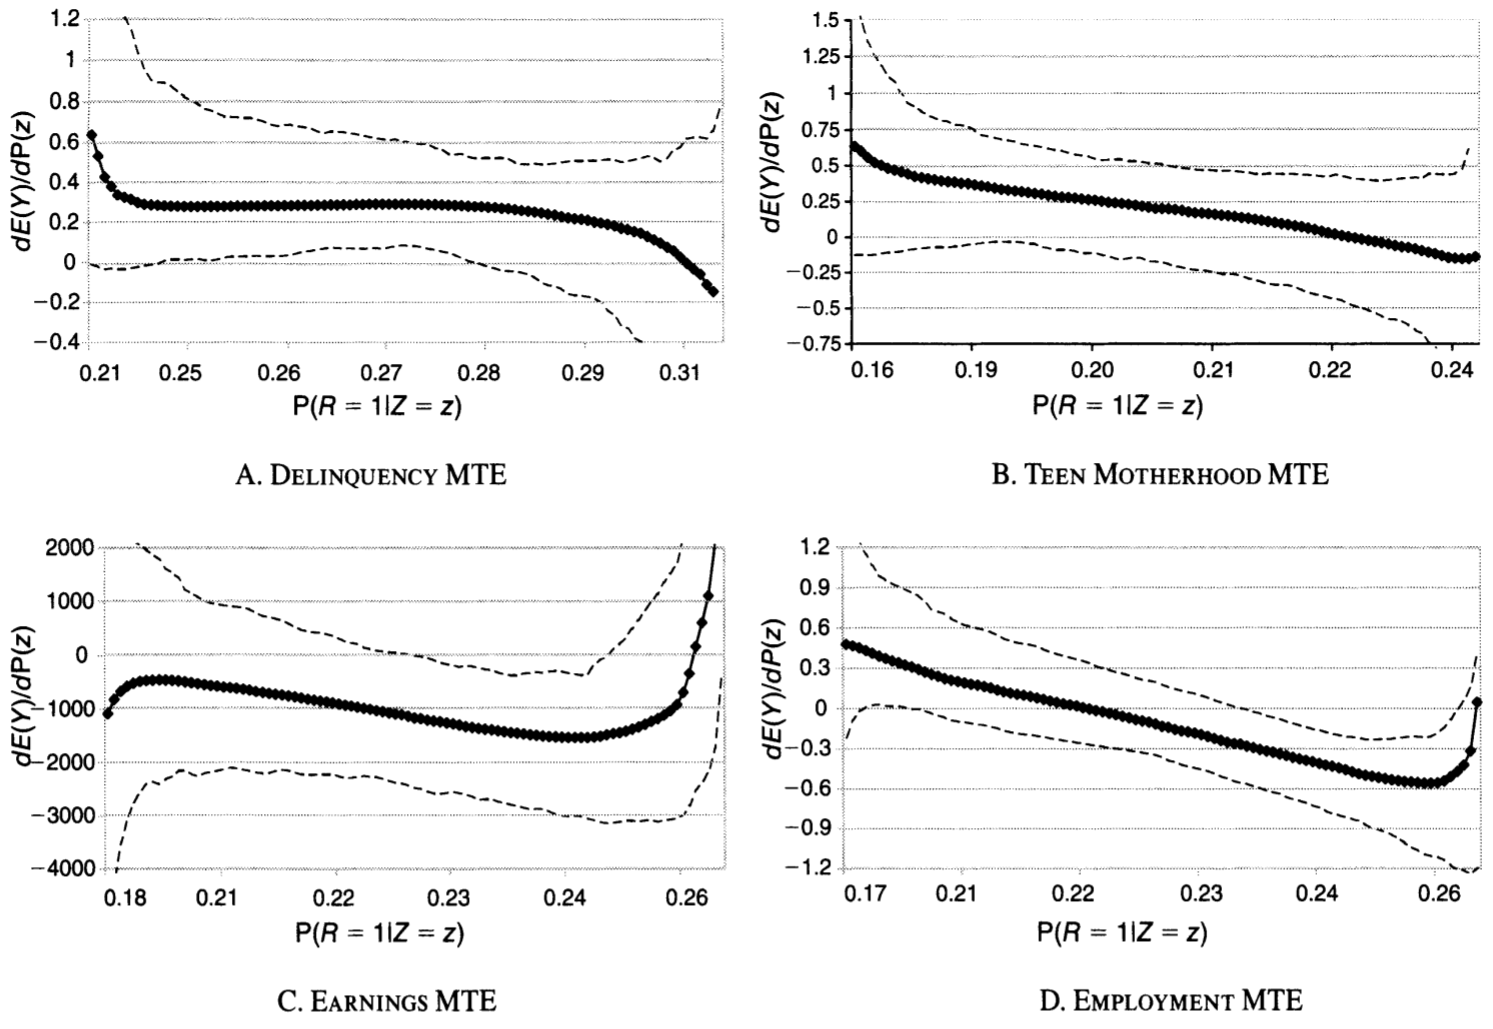
\includegraphics[scale=0.3]{./lecture_includes/doyle_mtes.png}
\end{center}
\end{frame}

\begin{frame}{Local Instrumental Variables}
Heckman (2000) shows that MTEs are identified by ``local IV'':\smallskip
\begin{align*}
E[Y_i(1)-Y_i(0)\mid U_i=p]=\frac{\partial E[Y_i\mid p(Z_i)=p]}{\partial p}
\end{align*}
under natural extensions of Imbens and Angrist (1994)\smallskip\pause{}
\begin{itemize}
\item Suggests we flexibly estimate $p(z)=Pr(D_i=1\mid Z_i=z)$, $E[Y_i\mid p(Z_i)]$, and then take the derivative of the latter\smallskip
\item In practice this is often done parametrically, and with controls
\end{itemize}

\end{frame}

\subsection{Discrete Instruments}
\begin{frame}{What if We Don't Have Continuous Instruments?}
A fascinating recent literature considers intermediate cases of Imbens-Angrist and Heckman-Vytlacil:\smallskip
\begin{itemize}
\item Discrete (binary/multivalued) $Z_i$, with parametric/shape restrictions to trace out (or maybe bound) the MTE curve\smallskip
\item Effectively using a model to ``extrapolate'' from local variation, maybe to identify more policy-relevant parameters
\end{itemize}\medskip\pause{}
Some examples: Brinch et al. (2017),  Mogstad et al. (2018), Kline and Walters (2019), Hull (2020), Arnold et al. (2021), Kowalski (2022)...\smallskip
\begin{itemize}
\item Lots more to do here (especially on the practical side)
\end{itemize}
\end{frame}

\begin{frame}{How Parametric ``Heckit'' Models Extrapolate LATEs}
\vspace{-0.3cm}
\begin{center}
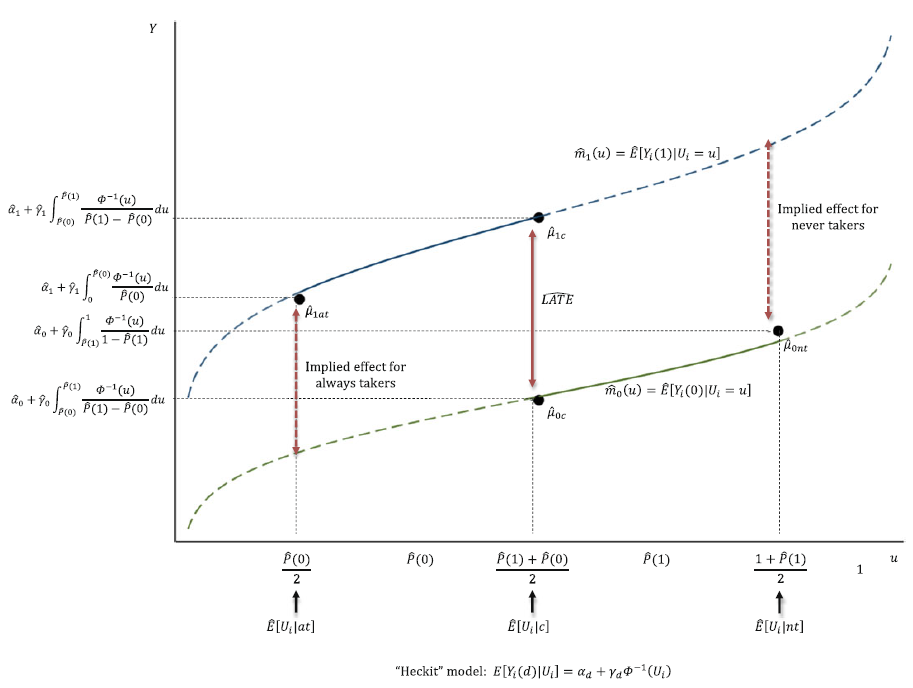
\includegraphics[scale=0.4]{./lecture_includes/kline_walters.png}
\end{center}
Source: Kline and Walters (2019) 
\end{frame}

\end{document}
